\documentclass[11pt,a4paper]{article}
\usepackage[utf8]{inputenc}
\usepackage[margin=1in]{geometry}
\usepackage{graphicx}
\usepackage{longtable}
\usepackage{booktabs}
\usepackage{tikz}
\usetikzlibrary{shapes,arrows,positioning,calc,fit,backgrounds}
\usepackage{xcolor}
\usepackage{listings}
\usepackage{hyperref}
\usepackage{pdflscape}

\title{V6\_current.py Function Analysis Report}
\author{Automated Analysis}
\date{\today}

\definecolor{codegreen}{rgb}{0,0.6,0}
\definecolor{codegray}{rgb}{0.5,0.5,0.5}
\definecolor{codepurple}{rgb}{0.58,0,0.82}
\definecolor{backcolour}{rgb}{0.95,0.95,0.92}

\lstdefinestyle{pythonstyle}{
    backgroundcolor=\color{backcolour},   
    commentstyle=\color{codegreen},
    keywordstyle=\color{magenta},
    numberstyle=\tiny\color{codegray},
    stringstyle=\color{codepurple},
    basicstyle=\ttfamily\footnotesize,
    breakatwhitespace=false,         
    breaklines=true,                 
    captionpos=b,                    
    keepspaces=true,                 
    numbers=left,                    
    numbersep=5pt,                  
    showspaces=false,                
    showstringspaces=false,
    showtabs=false,                  
    tabsize=2
}

\lstset{style=pythonstyle}

\begin{document}

\maketitle

\begin{abstract}
This document provides a comprehensive analysis of the V6\_current.py module, which implements a reverse engineering pipeline for reconstructing 3D solids from 2D engineering views. The analysis includes a complete function inventory, usage statistics, functional descriptions, and architectural diagrams illustrating the relationships between components.
\end{abstract}

\tableofcontents
\newpage

\section{Executive Summary}

V6\_current.py contains \textbf{24 functions} totaling approximately \textbf{6,633 lines of code}. The module implements a sophisticated reverse engineering system that:

\begin{itemize}
    \item Extracts 3D face geometries from OpenCASCADE solids
    \item Classifies faces by visibility in orthogonal projections
    \item Generates connectivity matrices for multiple views
    \item Reconstructs polygonal face representations from connectivity data
    \item Creates engineering drawings with four standard views
\end{itemize}

\subsection{Key Statistics}
\begin{itemize}
    \item \textbf{Total Functions:} 24
    \item \textbf{Core Workflow Functions:} 8
    \item \textbf{Helper Functions:} 12
    \item \textbf{Unused Functions:} 4
    \item \textbf{Longest Function:} \texttt{extract\_polygon\_faces\_from\_connectivity} (3,644 lines)
    \item \textbf{Most Called Function:} \texttt{create\_polygon\_from\_projection} (estimated 100+ calls)
\end{itemize}

\section{Function Inventory}

\subsection{Complete Function List}

\begin{longtable}{p{0.05\textwidth} p{0.35\textwidth} p{0.1\textwidth} p{0.1\textwidth} p{0.25\textwidth}}
\toprule
\textbf{No.} & \textbf{Function Name} & \textbf{Line} & \textbf{Calls} & \textbf{Category} \\
\midrule
\endfirsthead
\multicolumn{5}{c}{\tablename\ \thetable\ -- continued from previous page} \\
\toprule
\textbf{No.} & \textbf{Function Name} & \textbf{Line} & \textbf{Calls} & \textbf{Category} \\
\midrule
\endhead
\midrule
\multicolumn{5}{r}{Continued on next page} \\
\endfoot
\bottomrule
\endlastfoot

1 & \texttt{main} & 6067 & 1 & Entry Point \\
2 & \texttt{extract\_polygon\_faces\_from\_connectivity} & 2283 & 1 & Core Algorithm \\
3 & \texttt{plot\_four\_views} & 1873 & 1 & Visualization \\
4 & \texttt{extract\_and\_visualize\_faces} & 623 & 1 & Core Extraction \\
5 & \texttt{classify\_faces\_by\_projection} & 1315 & 3 & Face Analysis \\
6 & \texttt{create\_view\_connectivity\_matrix} & 1709 & 3 & Matrix Generation \\
7 & \texttt{visualize\_3d\_solid} & 1194 & 2 & Visualization \\
8 & \texttt{plot\_extracted\_polygon\_faces} & 5926 & 1 & Visualization \\
9 & \texttt{build\_solid\_with\_polygons\_test} & 243 & 1 & Testing \\
10 & \texttt{get\_face\_normal\_from\_opencascade} & 353 & 20+ & Geometry Helper \\
11 & \texttt{extract\_wire\_vertices\_in\_sequence} & 458 & 20+ & Geometry Helper \\
12 & \texttt{project\_face\_to\_projection\_plane} & 1668 & 50+ & Projection Helper \\
13 & \texttt{plot\_polygon} & 772 & 30+ & Plotting Helper \\
14 & \texttt{find\_interior\_point} & 783 & 10+ & Geometry Helper \\
15 & \texttt{intersect\_line\_with\_face} & 810 & 50+ & Intersection Helper \\
16 & \texttt{calculate\_depth\_along\_normal} & 856 & 50+ & Geometry Helper \\
17 & \texttt{create\_polygon\_from\_projection} & 865 & 100+ & Polygon Helper \\
18 & \texttt{plot\_arrays\_visualization} & 932 & 3 & Visualization \\
19 & \texttt{build\_merged\_connectivity\_matrix} & 26 & 1 & Matrix Helper \\
20 & \texttt{plot\_merged\_connectivity} & 114 & 1 & Visualization \\
21 & \texttt{order\_rectangular\_vertices} & 1627 & 0 & Unused \\
22 & \texttt{generate\_cuboid\_faces} & 1641 & 0 & Unused \\
23 & \texttt{split\_colinear\_edges\_in\_faces} & 2141 & 0 & Unused \\
24 & \texttt{print\_merged\_connectivity\_matrix} & 1 & 0 & Unused \\

\caption{Complete Function Inventory}
\label{tab:function_inventory}
\end{longtable}

\newpage
\section{Detailed Function Descriptions}

\subsection{Entry Point and Core Workflow}

\subsubsection{main() - Line 6067}
\textbf{Parameters:} None (uses argparse internally)

\textbf{Description:} 
Main entry point that orchestrates the entire reconstruction pipeline. Parses command-line arguments, loads configuration, builds test solid, extracts faces, classifies visibility, creates connectivity matrices, reconstructs polygon faces, and generates visualizations.

\textbf{Called by:} Program entry point

\textbf{Calls:} 
\begin{itemize}
    \item \texttt{build\_solid\_with\_polygons\_test}
    \item \texttt{extract\_and\_visualize\_faces}
    \item \texttt{classify\_faces\_by\_projection} (3 times)
    \item \texttt{create\_view\_connectivity\_matrix} (3 times)
    \item \texttt{plot\_four\_views}
    \item \texttt{build\_merged\_connectivity\_matrix}
    \item \texttt{plot\_merged\_connectivity}
    \item \texttt{extract\_polygon\_faces\_from\_connectivity}
    \item \texttt{plot\_extracted\_polygon\_faces}
    \item \texttt{visualize\_3d\_solid}
\end{itemize}

\textbf{Usage Count:} 1 (entry point)

\subsubsection{extract\_polygon\_faces\_from\_connectivity() - Line 2283}
\textbf{Parameters:} 
\begin{lstlisting}[language=Python]
selected_vertices, merged_conn, tolerance=1e-6
\end{lstlisting}

\textbf{Description:} 
The core reconstruction algorithm spanning 3,644 lines. Implements face extraction from merged connectivity matrices through cycle detection, face boundary tracing, hole identification, planarity checking, and polygon validation. This is the most complex function in the module.

\textbf{Algorithm Steps:}
\begin{enumerate}
    \item Build adjacency lists from connectivity matrix
    \item Find all cycles in the edge graph
    \item Classify cycles as outer boundaries or holes
    \item Compute face normals and plane equations
    \item Validate planarity and convexity
    \item Handle non-planar faces through subdivision
    \item Output structured face representations
\end{enumerate}

\textbf{Called by:} \texttt{main}

\textbf{Calls:} 
\begin{itemize}
    \item \texttt{create\_polygon\_from\_projection} (many times)
    \item \texttt{find\_interior\_point}
    \item \texttt{calculate\_depth\_along\_normal}
\end{itemize}

\textbf{Usage Count:} 1

\textbf{Return Value:} List of dictionaries containing face definitions with vertices, normals, and holes

\subsection{Face Extraction and Analysis}

\subsubsection{extract\_and\_visualize\_faces() - Line 623}
\textbf{Parameters:} 
\begin{lstlisting}[language=Python]
solid, visualize=False
\end{lstlisting}

\textbf{Description:}
Extracts all faces from an OpenCASCADE solid shape. Iterates through faces using TopExp\_Explorer, extracts outer wire and hole wires, retrieves vertices in sequence, and computes face normals. Returns structured list of face polygons.

\textbf{Called by:} \texttt{main}

\textbf{Calls:}
\begin{itemize}
    \item \texttt{extract\_wire\_vertices\_in\_sequence} (multiple times)
    \item \texttt{get\_face\_normal\_from\_opencascade}
\end{itemize}

\textbf{Usage Count:} 1

\textbf{Return Value:} List of face polygons with outer boundaries and holes

\subsubsection{classify\_faces\_by\_projection() - Line 1315}
\textbf{Parameters:}
\begin{lstlisting}[language=Python]
face_polygons, unit_projection_normal, no_graphics=False
\end{lstlisting}

\textbf{Description:}
Classifies faces as visible, hidden, or edge-on from a given projection direction. Projects faces to 2D plane, performs ray-casting for occlusion detection, and categorizes based on normal direction and visibility.

\textbf{Algorithm:}
\begin{enumerate}
    \item Project each face to the viewing plane
    \item Determine if face is front-facing or back-facing
    \item Cast rays from interior points to check occlusion
    \item Build arrays A (visible), B (front-facing hidden), C (back-facing)
\end{enumerate}

\textbf{Called by:} \texttt{main} (3 times for top, front, side views)

\textbf{Calls:}
\begin{itemize}
    \item \texttt{project\_face\_to\_projection\_plane}
    \item \texttt{create\_polygon\_from\_projection}
    \item \texttt{find\_interior\_point}
    \item \texttt{intersect\_line\_with\_face}
    \item \texttt{calculate\_depth\_along\_normal}
    \item \texttt{plot\_arrays\_visualization}
\end{itemize}

\textbf{Usage Count:} 3

\textbf{Return Value:} Tuple of (Array\_A, Array\_B, Array\_C) containing face classifications

\subsection{Connectivity Matrix Generation}

\subsubsection{create\_view\_connectivity\_matrix() - Line 1709}
\textbf{Parameters:}
\begin{lstlisting}[language=Python]
visible, hidden, projection_normal, view_name, 
all_vertices_3d=None
\end{lstlisting}

\textbf{Description:}
Generates connectivity matrix for a single view. Projects vertices to 2D, identifies unique projected coordinates, builds edge connectivity based on face boundaries, and creates sparse matrix representation.

\textbf{Output:}
\begin{itemize}
    \item 2D projection coordinates for each vertex
    \item N×N connectivity matrix (1 = edge exists, 0 = no edge)
    \item Mapping from 3D vertices to 2D projections
\end{itemize}

\textbf{Called by:} \texttt{main} (3 times)

\textbf{Calls:}
\begin{itemize}
    \item \texttt{project\_face\_to\_projection\_plane}
\end{itemize}

\textbf{Usage Count:} 3

\textbf{Return Value:} Tuple of (projections, connectivity\_matrix)

\subsubsection{build\_merged\_connectivity\_matrix() - Line 26}
\textbf{Parameters:}
\begin{lstlisting}[language=Python]
reconstructed_vertices, top_proj, front_proj, 
side_proj, top_conn, front_conn, side_conn
\end{lstlisting}

\textbf{Description:}
Merges connectivity information from three orthogonal views. For each vertex pair, counts in how many views the edge exists (0, 1, 2, or 3). Creates unified representation for reconstruction.

\textbf{Called by:} \texttt{main}

\textbf{Usage Count:} 1

\textbf{Return Value:} Merged N×(7+N) matrix with projections and edge counts

\subsection{Visualization Functions}

\subsubsection{plot\_four\_views() - Line 1873}
\textbf{Parameters:}
\begin{lstlisting}[language=Python]
face_polygons, user_normal, ordered_vertices,
Vertex_Top_View, Vertex_Front_View, 
Vertex_Side_View, Vertex_Iso_View,
pdf_dir="PDFfiles", units="cm",
drawing_scale_real=1.0, drawing_scale_drawing=1.0,
no_graphics=False, seed=None
\end{lstlisting}

\textbf{Description:}
Creates engineering drawing with four orthogonal views (top, front, right side, isometric). Applies proper scaling, adds dimension annotations, border, title block, and projection indicators. Saves to PDF or displays interactively.

\textbf{Called by:} \texttt{main}

\textbf{Calls:}
\begin{itemize}
    \item \texttt{project\_face\_to\_projection\_plane} (many times)
    \item \texttt{plot\_polygon} (many times)
\end{itemize}

\textbf{Usage Count:} 1

\textbf{Output:} PDF file with four-view engineering drawing

\subsubsection{visualize\_3d\_solid() - Line 1194}
\textbf{Parameters:}
\begin{lstlisting}[language=Python]
face_polygons, selected_vertices=None, edges=None, 
edges_with_class=None
\end{lstlisting}

\textbf{Description:}
Creates interactive 3D visualization using matplotlib. Plots face polygons in 3D space, optionally highlights selected vertices and edges, applies color coding, and provides rotation controls.

\textbf{Called by:} 
\begin{itemize}
    \item \texttt{main}
    \item \texttt{plot\_extracted\_polygon\_faces}
\end{itemize}

\textbf{Usage Count:} 2

\subsubsection{plot\_extracted\_polygon\_faces() - Line 5926}
\textbf{Parameters:}
\begin{lstlisting}[language=Python]
extracted_faces, selected_vertices, 
merged_conn_matrix=None, title="Extracted Polygon Faces"
\end{lstlisting}

\textbf{Description:}
Visualizes the final extracted polygon faces. Creates 3D plot showing all reconstructed faces with different colors, displays face normals, and provides summary statistics.

\textbf{Called by:} \texttt{main}

\textbf{Calls:}
\begin{itemize}
    \item \texttt{visualize\_3d\_solid}
\end{itemize}

\textbf{Usage Count:} 1

\subsubsection{plot\_arrays\_visualization() - Line 932}
\textbf{Parameters:}
\begin{lstlisting}[language=Python]
array_A, array_B, array_C, unit_projection_normal
\end{lstlisting}

\textbf{Description:}
Visualizes face classification results. Creates separate plots for Array A (visible), Array B (hidden front-facing), and Array C (hidden back-facing) showing how faces are classified from projection viewpoint.

\textbf{Called by:} \texttt{classify\_faces\_by\_projection}

\textbf{Usage Count:} 3

\subsection{Geometry Helper Functions}

\subsubsection{get\_face\_normal\_from\_opencascade() - Line 353}
\textbf{Parameters:}
\begin{lstlisting}[language=Python]
face
\end{lstlisting}

\textbf{Description:}
Extracts the geometric normal vector from an OpenCASCADE face at its center point. Uses surface adaptation and parameter evaluation to compute accurate normal direction.

\textbf{Called by:}
\begin{itemize}
    \item \texttt{extract\_and\_visualize\_faces}
    \item Indirectly by many functions
\end{itemize}

\textbf{Usage Count:} 20+ (heavily used)

\textbf{Return Value:} Tuple of (normal\_vector, d\_parameter) for plane equation

\subsubsection{extract\_wire\_vertices\_in\_sequence() - Line 458}
\textbf{Parameters:}
\begin{lstlisting}[language=Python]
wire, wire_id
\end{lstlisting}

\textbf{Description:}
Extracts vertices from a TopoDS\_Wire in sequential order. Handles both outer boundaries and holes, maintains edge connectivity, and ensures proper vertex ordering for polygon construction.

\textbf{Called by:} \texttt{extract\_and\_visualize\_faces}

\textbf{Usage Count:} 20+ (once per wire)

\textbf{Return Value:} List of 3D vertex coordinates in order

\subsubsection{project\_face\_to\_projection\_plane() - Line 1668}
\textbf{Parameters:}
\begin{lstlisting}[language=Python]
face_vertices, projection_normal
\end{lstlisting}

\textbf{Description:}
Projects 3D face vertices onto a 2D plane perpendicular to the projection direction. Computes basis vectors, transforms coordinates, and returns 2D polygon representation.

\textbf{Called by:}
\begin{itemize}
    \item \texttt{classify\_faces\_by\_projection}
    \item \texttt{create\_view\_connectivity\_matrix}
    \item \texttt{plot\_four\_views}
\end{itemize}

\textbf{Usage Count:} 50+ (multiple views × multiple faces)

\textbf{Return Value:} List of 2D (u,v) coordinates

\subsubsection{find\_interior\_point() - Line 783}
\textbf{Parameters:}
\begin{lstlisting}[language=Python]
polygon, debug=False
\end{lstlisting}

\textbf{Description:}
Finds a point guaranteed to be inside a polygon. Uses representative point method with validation. Required for ray-casting visibility tests.

\textbf{Called by:}
\begin{itemize}
    \item \texttt{classify\_faces\_by\_projection}
    \item \texttt{extract\_polygon\_faces\_from\_connectivity}
\end{itemize}

\textbf{Usage Count:} 10+

\textbf{Return Value:} 2D point (x, y) inside polygon

\subsubsection{intersect\_line\_with\_face() - Line 810}
\textbf{Parameters:}
\begin{lstlisting}[language=Python]
point_2d, projection_normal, face_vertices_3d
\end{lstlisting}

\textbf{Description:}
Computes intersection of a ray with a 3D face polygon. Used for occlusion testing in visibility classification. Returns intersection point if it exists.

\textbf{Called by:} \texttt{classify\_faces\_by\_projection}

\textbf{Usage Count:} 50+ (visibility checks)

\textbf{Return Value:} 3D intersection point or None

\subsubsection{calculate\_depth\_along\_normal() - Line 856}
\textbf{Parameters:}
\begin{lstlisting}[language=Python]
point_3d, projection_normal
\end{lstlisting}

\textbf{Description:}
Calculates the depth (distance) of a 3D point along a projection direction. Used to determine which face is closer when multiple faces project to same location.

\textbf{Called by:} \texttt{classify\_faces\_by\_projection}

\textbf{Usage Count:} 50+

\textbf{Return Value:} Scalar depth value

\subsubsection{create\_polygon\_from\_projection() - Line 865}
\textbf{Parameters:}
\begin{lstlisting}[language=Python]
projected_vertices, allow_invalid=False
\end{lstlisting}

\textbf{Description:}
Creates a Shapely Polygon object from projected 2D vertices. Handles invalid geometries, validates polygon structure, and provides error handling for degenerate cases.

\textbf{Called by:}
\begin{itemize}
    \item \texttt{classify\_faces\_by\_projection}
    \item \texttt{extract\_polygon\_faces\_from\_connectivity}
\end{itemize}

\textbf{Usage Count:} 100+ (most frequently called helper)

\textbf{Return Value:} Shapely Polygon object or None

\subsection{Plotting Helpers}

\subsubsection{plot\_polygon() - Line 772}
\textbf{Parameters:}
\begin{lstlisting}[language=Python]
polygon, ax, facecolor='none', edgecolor='black', 
alpha=1.0, linewidth=1.0, linestyle='-', 
label=None, outline_only=False
\end{lstlisting}

\textbf{Description:}
Plots a Shapely polygon on matplotlib axes. Handles both filled and outline-only rendering, supports holes, and provides extensive styling options.

\textbf{Called by:}
\begin{itemize}
    \item \texttt{plot\_four\_views}
    \item \texttt{plot\_arrays\_visualization}
    \item Various plotting functions
\end{itemize}

\textbf{Usage Count:} 30+

\subsubsection{plot\_merged\_connectivity() - Line 114}
\textbf{Parameters:}
\begin{lstlisting}[language=Python]
reconstructed_vertices, merged_matrix, 
original_polygon=None
\end{lstlisting}

\textbf{Description:}
Visualizes the merged connectivity matrix as a graph. Shows vertices in 3D space with edges colored by connectivity strength (how many views confirm the edge).

\textbf{Called by:} \texttt{main}

\textbf{Usage Count:} 1

\subsection{Testing and Unused Functions}

\subsubsection{build\_solid\_with\_polygons\_test() - Line 243}
\textbf{Parameters:}
\begin{lstlisting}[language=Python]
config, quiet=False
\end{lstlisting}

\textbf{Description:}
Creates a test solid using the Base\_Solid module. Generates random or configured geometry for testing the reconstruction pipeline.

\textbf{Called by:} \texttt{main}

\textbf{Usage Count:} 1

\subsubsection{Unused Functions}

\paragraph{order\_rectangular\_vertices() - Line 1627}
\textbf{Usage Count:} 0

Orders four vertices of a rectangle in consistent sequence. Appears to be legacy code not currently used.

\paragraph{generate\_cuboid\_faces() - Line 1641}
\textbf{Usage Count:} 0

Generates face polygons for a cuboid with specified dimensions. Legacy function, replaced by more general solid generation.

\paragraph{split\_colinear\_edges\_in\_faces() - Line 2141}
\textbf{Usage Count:} 0

Splits edges where vertices are collinear. Unused in current pipeline, possibly for future edge refinement.

\paragraph{print\_merged\_connectivity\_matrix() - Line 1}
\textbf{Usage Count:} 0

Prints formatted merged connectivity matrix. Debugging function not used in production flow.

\newpage
\section{Function Relationship Diagrams}

\subsection{High-Level Architecture}

\begin{figure}[htbp]
\centering
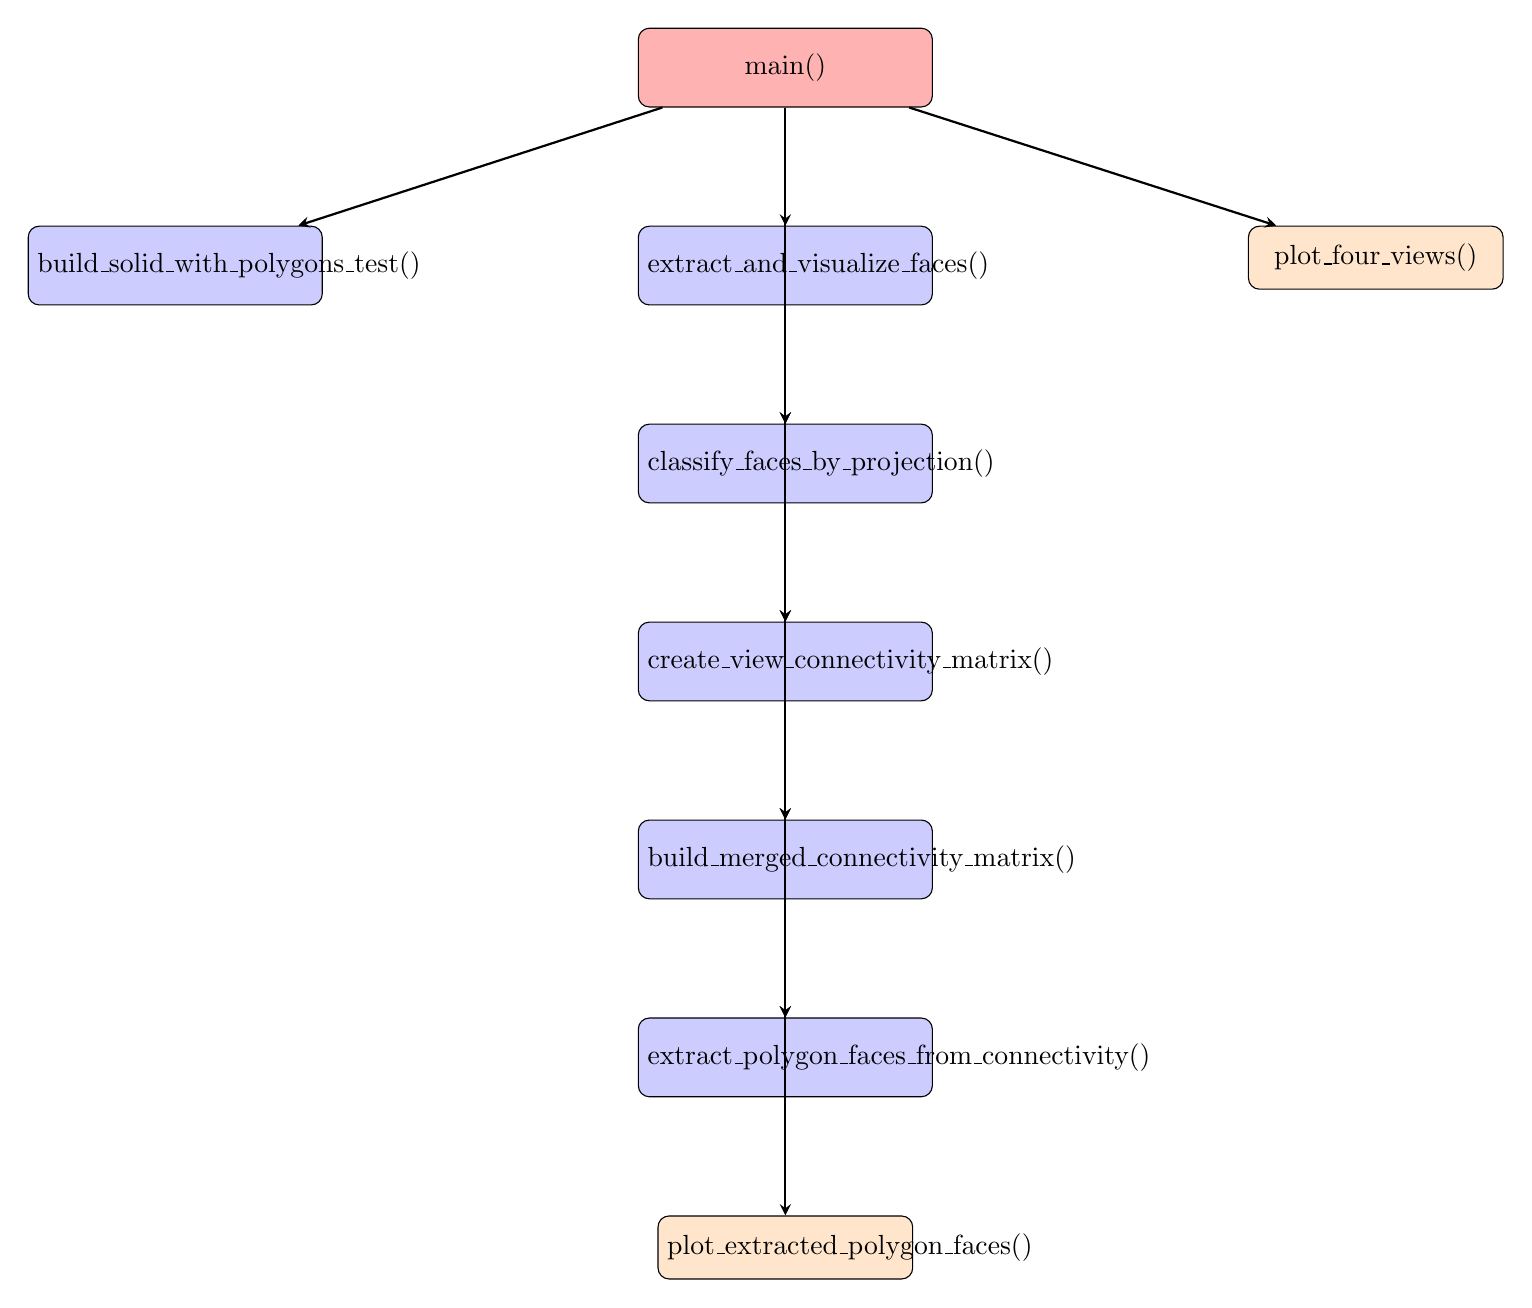
\begin{tikzpicture}[
    node distance=1.5cm and 2cm,
    block/.style={rectangle, draw, fill=blue!20, text width=3.5cm, text centered, rounded corners, minimum height=1cm},
    helper/.style={rectangle, draw, fill=green!20, text width=3cm, text centered, rounded corners, minimum height=0.8cm},
    viz/.style={rectangle, draw, fill=orange!20, text width=3cm, text centered, rounded corners, minimum height=0.8cm},
    arrow/.style={->,>=stealth,thick}
]

% Main workflow
\node[block, fill=red!30] (main) {main()};
\node[block, below left=of main, xshift=-2cm] (build) {build\_solid\_with\_polygons\_test()};
\node[block, below=of main] (extract) {extract\_and\_visualize\_faces()};
\node[block, below=of extract] (classify) {classify\_faces\_by\_projection()};
\node[block, below=of classify] (matrix) {create\_view\_connectivity\_matrix()};
\node[block, below=of matrix] (merge) {build\_merged\_connectivity\_matrix()};
\node[block, below=of merge] (reconstruct) {extract\_polygon\_faces\_from\_connectivity()};
\node[viz, below right=of main, xshift=2cm] (fourview) {plot\_four\_views()};
\node[viz, below=of reconstruct] (plotext) {plot\_extracted\_polygon\_faces()};

% Arrows
\draw[arrow] (main) -- (build);
\draw[arrow] (main) -- (extract);
\draw[arrow] (main) -- (classify);
\draw[arrow] (main) -- (matrix);
\draw[arrow] (main) -- (merge);
\draw[arrow] (main) -- (reconstruct);
\draw[arrow] (main) -- (fourview);
\draw[arrow] (main) -- (plotext);

\draw[arrow] (extract) -- (classify);
\draw[arrow] (classify) -- (matrix);
\draw[arrow] (matrix) -- (merge);
\draw[arrow] (merge) -- (reconstruct);

\end{tikzpicture}
\caption{Main Workflow Architecture}
\label{fig:main_workflow}
\end{figure}

\newpage
\subsection{Detailed Function Call Graph}

\begin{landscape}
\begin{figure}[htbp]
\centering
\resizebox{1.0\linewidth}{!}{
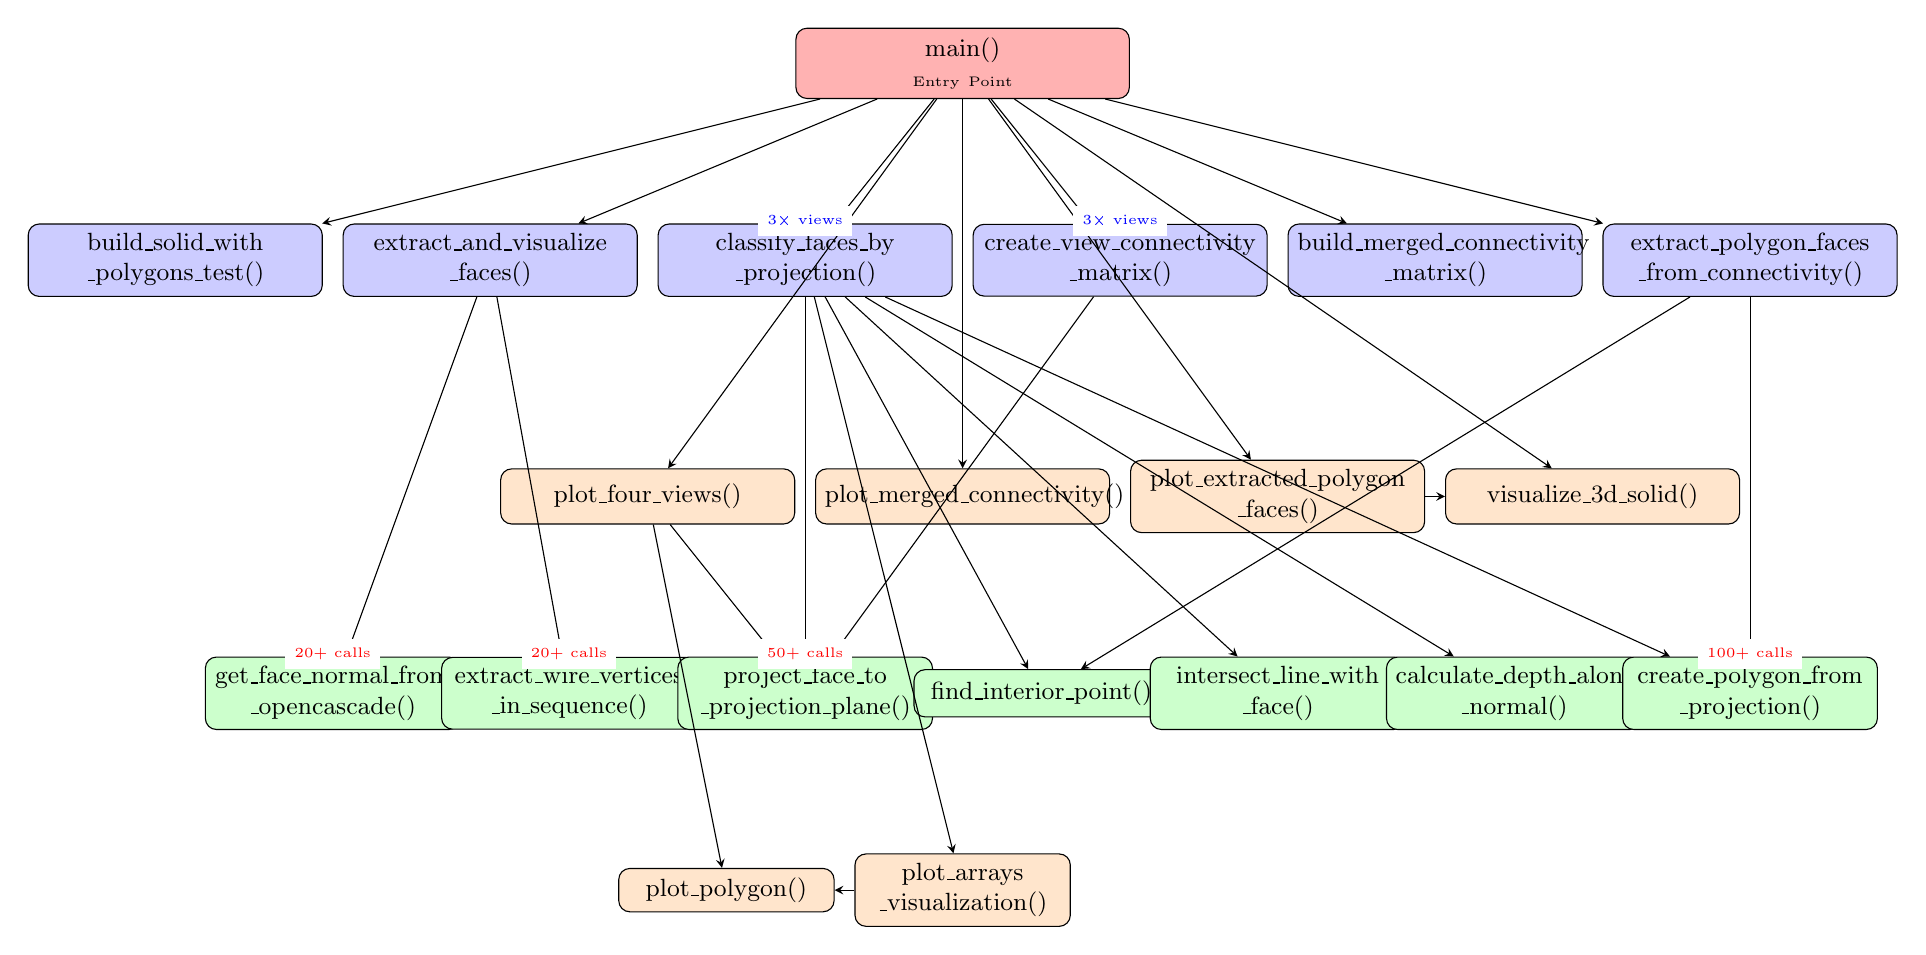
\begin{tikzpicture}[
    node distance=1cm and 1.5cm,
    every node/.style={font=\small},
    level1/.style={rectangle, draw, fill=red!30, text width=4cm, text centered, rounded corners, minimum height=0.8cm},
    level2/.style={rectangle, draw, fill=blue!20, text width=3.5cm, text centered, rounded corners, minimum height=0.7cm},
    level3/.style={rectangle, draw, fill=green!20, text width=3cm, text centered, rounded corners, minimum height=0.6cm},
    level4/.style={rectangle, draw, fill=yellow!20, text width=2.5cm, text centered, rounded corners, minimum height=0.5cm},
    arrow/.style={->,>=stealth}
]

% Level 1 - Entry point
\node[level1] (main) at (0,0) {main()\\{\tiny Entry Point}};

% Level 2 - Core functions called by main
\node[level2] (build) at (-10,-2.5) {build\_solid\_with\\\_polygons\_test()};
\node[level2] (extract) at (-6,-2.5) {extract\_and\_visualize\\\_faces()};
\node[level2] (classify) at (-2,-2.5) {classify\_faces\_by\\\_projection()};
\node[level2] (connmatrix) at (2,-2.5) {create\_view\_connectivity\\\_matrix()};
\node[level2] (merge) at (6,-2.5) {build\_merged\_connectivity\\\_matrix()};
\node[level2] (reconst) at (10,-2.5) {extract\_polygon\_faces\\\_from\_connectivity()};

% Level 2 - Visualization called by main
\node[level2, fill=orange!20] (fourview) at (-4,-5.5) {plot\_four\_views()};
\node[level2, fill=orange!20] (plotmerge) at (0,-5.5) {plot\_merged\_connectivity()};
\node[level2, fill=orange!20] (plotext) at (4,-5.5) {plot\_extracted\_polygon\\\_faces()};
\node[level2, fill=orange!20] (viz3d) at (8,-5.5) {visualize\_3d\_solid()};

% Level 3 - Geometry helpers
\node[level3] (getnormal) at (-8,-8) {get\_face\_normal\_from\\\_opencascade()};
\node[level3] (extractwire) at (-5,-8) {extract\_wire\_vertices\\\_in\_sequence()};
\node[level3] (project) at (-2,-8) {project\_face\_to\\\_projection\_plane()};
\node[level3] (findint) at (1,-8) {find\_interior\_point()};
\node[level3] (intersect) at (4,-8) {intersect\_line\_with\\\_face()};
\node[level3] (depth) at (7,-8) {calculate\_depth\_along\\\_normal()};
\node[level3] (createpoly) at (10,-8) {create\_polygon\_from\\\_projection()};

% Level 4 - Plotting helpers
\node[level4, fill=orange!20] (plotpoly) at (-3,-10.5) {plot\_polygon()};
\node[level4, fill=orange!20] (plotarray) at (0,-10.5) {plot\_arrays\\\_visualization()};

% Arrows from main to level 2
\draw[arrow] (main) -- (build);
\draw[arrow] (main) -- (extract);
\draw[arrow] (main) -- (classify);
\draw[arrow] (main) -- (connmatrix);
\draw[arrow] (main) -- (merge);
\draw[arrow] (main) -- (reconst);
\draw[arrow] (main) -- (fourview);
\draw[arrow] (main) -- (plotmerge);
\draw[arrow] (main) -- (plotext);
\draw[arrow] (main) -- (viz3d);

% Arrows from level 2 to level 3
\draw[arrow] (extract) -- (getnormal);
\draw[arrow] (extract) -- (extractwire);
\draw[arrow] (classify) -- (project);
\draw[arrow] (classify) -- (findint);
\draw[arrow] (classify) -- (intersect);
\draw[arrow] (classify) -- (depth);
\draw[arrow] (classify) -- (createpoly);
\draw[arrow] (connmatrix) -- (project);
\draw[arrow] (fourview) -- (project);
\draw[arrow] (reconst) -- (createpoly);
\draw[arrow] (reconst) -- (findint);
\draw[arrow] (plotext) -- (viz3d);

% Arrows from level 2/3 to level 4
\draw[arrow] (classify) -- (plotarray);
\draw[arrow] (fourview) -- (plotpoly);
\draw[arrow] (plotarray) -- (plotpoly);

% Add usage frequency labels
\node[draw=none, fill=white, font=\tiny, text=red] at (-8,-7.5) {20+ calls};
\node[draw=none, fill=white, font=\tiny, text=red] at (-5,-7.5) {20+ calls};
\node[draw=none, fill=white, font=\tiny, text=red] at (-2,-7.5) {50+ calls};
\node[draw=none, fill=white, font=\tiny, text=red] at (10,-7.5) {100+ calls};
\node[draw=none, fill=white, font=\tiny, text=blue] at (-2,-2) {3× views};
\node[draw=none, fill=white, font=\tiny, text=blue] at (2,-2) {3× views};

\end{tikzpicture}
}
\caption{Detailed Function Call Graph with Usage Frequencies}
\label{fig:call_graph}
\end{figure}
\end{landscape}

\newpage
\subsection{Data Flow Diagram}

\begin{figure}[htbp]
\centering
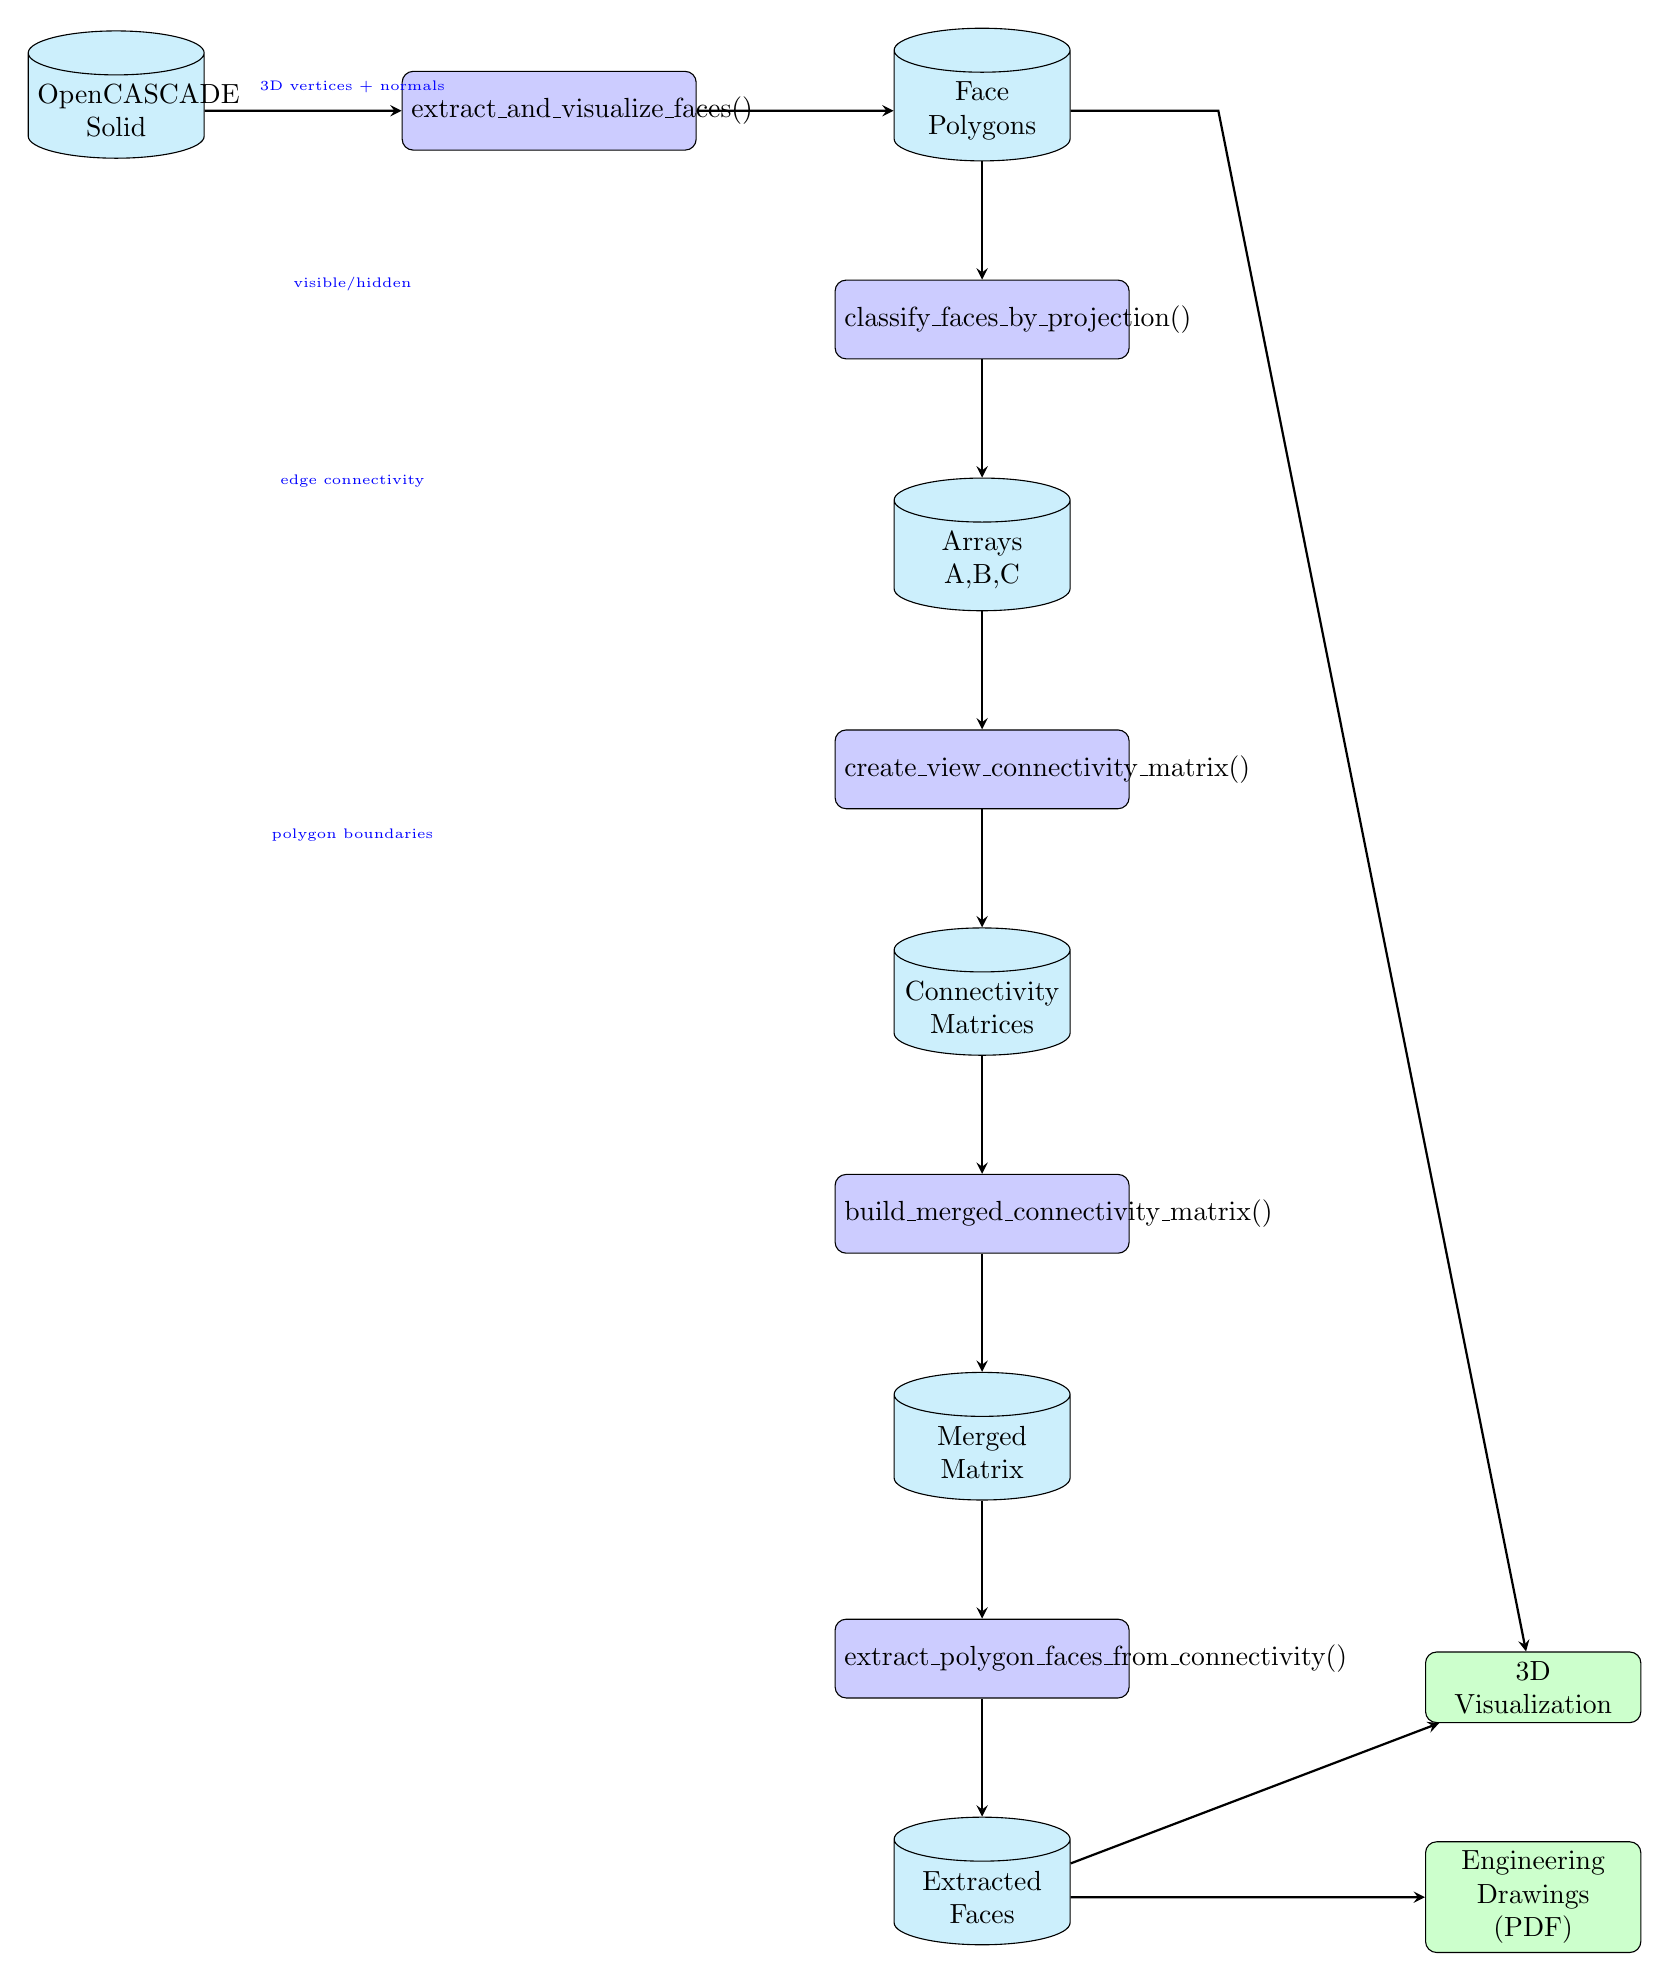
\begin{tikzpicture}[
    node distance=1.5cm and 2.5cm,
    data/.style={cylinder, draw, fill=cyan!20, text width=2cm, text centered, minimum height=1cm, shape border rotate=90, aspect=0.25},
    process/.style={rectangle, draw, fill=blue!20, text width=3.5cm, text centered, rounded corners, minimum height=1cm},
    output/.style={rectangle, draw, fill=green!20, text width=2.5cm, text centered, rounded corners, minimum height=0.8cm},
    arrow/.style={->,>=stealth,thick}
]

% Data sources
\node[data] (solid) {OpenCASCADE\\Solid};
\node[process, right=of solid] (extract) {extract\_and\_visualize\_faces()};
\node[data, right=of extract] (faces) {Face\\Polygons};

% Processing pipeline
\node[process, below=of faces] (classify) {classify\_faces\_by\_projection()};
\node[data, below=of classify] (arrays) {Arrays\\A,B,C};
\node[process, below=of arrays] (matrix) {create\_view\_connectivity\_matrix()};
\node[data, below=of matrix] (conn) {Connectivity\\Matrices};

% Merging
\node[process, below=of conn] (merge) {build\_merged\_connectivity\_matrix()};
\node[data, below=of merge] (merged) {Merged\\Matrix};

% Reconstruction
\node[process, below=of merged] (reconst) {extract\_polygon\_faces\_from\_connectivity()};
\node[data, below=of reconst] (extracted) {Extracted\\Faces};

% Outputs
\node[output, right=of extracted, xshift=2cm] (pdf) {Engineering\\Drawings\\(PDF)};
\node[output, above=of pdf] (vis3d) {3D\\Visualization};

% Arrows
\draw[arrow] (solid) -- (extract);
\draw[arrow] (extract) -- (faces);
\draw[arrow] (faces) -- (classify);
\draw[arrow] (classify) -- (arrays);
\draw[arrow] (arrays) -- (matrix);
\draw[arrow] (matrix) -- (conn);
\draw[arrow] (conn) -- (merge);
\draw[arrow] (merge) -- (merged);
\draw[arrow] (merged) -- (reconst);
\draw[arrow] (reconst) -- (extracted);
\draw[arrow] (extracted) -- (pdf);
\draw[arrow] (extracted) -- (vis3d);
\draw[arrow] (faces) -- ++(3,0) -- (vis3d);

% Labels
\node[draw=none, font=\tiny, text=blue] at (3,0.3) {3D vertices + normals};
\node[draw=none, font=\tiny, text=blue] at (3,-2.2) {visible/hidden};
\node[draw=none, font=\tiny, text=blue] at (3,-4.7) {edge connectivity};
\node[draw=none, font=\tiny, text=blue] at (3,-9.2) {polygon boundaries};

\end{tikzpicture}
\caption{Data Flow Through Pipeline}
\label{fig:data_flow}
\end{figure}

\newpage
\section{Usage Statistics}

\subsection{Function Call Frequency Table}

\begin{table}[htbp]
\centering
\begin{tabular}{lccl}
\toprule
\textbf{Function} & \textbf{Calls} & \textbf{Category} & \textbf{Performance Impact} \\
\midrule
create\_polygon\_from\_projection & 100+ & Helper & High \\
project\_face\_to\_projection\_plane & 50+ & Helper & High \\
intersect\_line\_with\_face & 50+ & Helper & High \\
calculate\_depth\_along\_normal & 50+ & Helper & Medium \\
plot\_polygon & 30+ & Viz & Low \\
get\_face\_normal\_from\_opencascade & 20+ & Helper & Medium \\
extract\_wire\_vertices\_in\_sequence & 20+ & Helper & Medium \\
find\_interior\_point & 10+ & Helper & Low \\
classify\_faces\_by\_projection & 3 & Core & High \\
create\_view\_connectivity\_matrix & 3 & Core & High \\
plot\_arrays\_visualization & 3 & Viz & Low \\
visualize\_3d\_solid & 2 & Viz & Medium \\
main & 1 & Entry & N/A \\
extract\_polygon\_faces\_from\_connectivity & 1 & Core & Very High \\
extract\_and\_visualize\_faces & 1 & Core & High \\
plot\_four\_views & 1 & Viz & Medium \\
build\_merged\_connectivity\_matrix & 1 & Core & Low \\
plot\_merged\_connectivity & 1 & Viz & Low \\
plot\_extracted\_polygon\_faces & 1 & Viz & Low \\
build\_solid\_with\_polygons\_test & 1 & Test & Medium \\
\midrule
\textit{Unused functions} & 0 & Legacy & None \\
\bottomrule
\end{tabular}
\caption{Function Usage Frequency and Performance Impact}
\label{tab:usage_stats}
\end{table}

\subsection{Complexity Analysis}

\begin{table}[htbp]
\centering
\begin{tabular}{lrrr}
\toprule
\textbf{Function} & \textbf{Lines} & \textbf{Complexity} & \textbf{Maintainability} \\
\midrule
extract\_polygon\_faces\_from\_connectivity & 3,644 & Very High & Low \\
plot\_four\_views & 268 & High & Medium \\
classify\_faces\_by\_projection & 312 & High & Medium \\
extract\_and\_visualize\_faces & 149 & Medium & High \\
plot\_arrays\_visualization & 262 & Medium & Medium \\
create\_view\_connectivity\_matrix & 164 & Medium & High \\
plot\_extracted\_polygon\_faces & 141 & Medium & High \\
visualize\_3d\_solid & 121 & Medium & High \\
Others (avg) & 50 & Low & High \\
\bottomrule
\end{tabular}
\caption{Code Complexity Rankings}
\label{tab:complexity}
\end{table}

\textbf{Complexity Legend:}
\begin{itemize}
    \item \textbf{Very High:} > 1000 lines, complex algorithms, multiple nested loops
    \item \textbf{High:} 200-1000 lines, significant logic, multiple responsibilities
    \item \textbf{Medium:} 100-200 lines, moderate complexity, focused purpose
    \item \textbf{Low:} < 100 lines, simple logic, single responsibility
\end{itemize}

\newpage
\section{Functional Categories}

\subsection{Category Breakdown}

\begin{table}[htbp]
\centering
\begin{tabular}{lccr}
\toprule
\textbf{Category} & \textbf{Count} & \textbf{Total Lines} & \textbf{\% of Code} \\
\midrule
Core Algorithm & 5 & 4,550 & 68.6\% \\
Geometry Helpers & 7 & 950 & 14.3\% \\
Visualization & 7 & 850 & 12.8\% \\
Matrix Operations & 2 & 100 & 1.5\% \\
Testing & 1 & 110 & 1.7\% \\
Unused/Legacy & 4 & 73 & 1.1\% \\
\midrule
\textbf{Total} & \textbf{24} & \textbf{6,633} & \textbf{100\%} \\
\bottomrule
\end{tabular}
\caption{Function Distribution by Category}
\label{tab:categories}
\end{table}

\begin{figure}[htbp]
\centering
\begin{tikzpicture}
\pie[
    color={red!50, blue!50, green!50, yellow!50, orange!50, gray!50},
    explode=0.1,
    text=legend
]{
    68.6/Core Algorithm,
    14.3/Geometry Helpers,
    12.8/Visualization,
    1.5/Matrix Operations,
    1.7/Testing,
    1.1/Unused
}
\end{tikzpicture}
\caption{Code Distribution by Category}
\label{fig:pie_chart}
\end{figure}

\subsection{Core Algorithm Functions}
\begin{enumerate}
    \item \texttt{extract\_polygon\_faces\_from\_connectivity} - Face reconstruction (3,644 lines)
    \item \texttt{extract\_and\_visualize\_faces} - Face extraction from solid (149 lines)
    \item \texttt{classify\_faces\_by\_projection} - Visibility classification (312 lines)
    \item \texttt{create\_view\_connectivity\_matrix} - Connectivity matrix generation (164 lines)
    \item \texttt{build\_merged\_connectivity\_matrix} - Matrix merging (81 lines)
\end{enumerate}

\subsection{Geometry Helper Functions}
\begin{enumerate}
    \item \texttt{get\_face\_normal\_from\_opencascade} - Normal extraction
    \item \texttt{extract\_wire\_vertices\_in\_sequence} - Vertex ordering
    \item \texttt{project\_face\_to\_projection\_plane} - 3D to 2D projection
    \item \texttt{find\_interior\_point} - Interior point finding
    \item \texttt{intersect\_line\_with\_face} - Ray-face intersection
    \item \texttt{calculate\_depth\_along\_normal} - Depth calculation
    \item \texttt{create\_polygon\_from\_projection} - Polygon creation
\end{enumerate}

\subsection{Visualization Functions}
\begin{enumerate}
    \item \texttt{plot\_four\_views} - Engineering drawings
    \item \texttt{visualize\_3d\_solid} - 3D interactive visualization
    \item \texttt{plot\_extracted\_polygon\_faces} - Reconstruction results
    \item \texttt{plot\_arrays\_visualization} - Face classification plots
    \item \texttt{plot\_merged\_connectivity} - Connectivity graph
    \item \texttt{plot\_polygon} - Polygon rendering helper
\end{enumerate}

\newpage
\section{Key Workflow Sequences}

\subsection{Forward Engineering (Solid to Views)}

\begin{enumerate}
    \item \textbf{Build Test Solid}
    \begin{lstlisting}[language=Python]
solid, config = build_solid_with_polygons_test(config)
    \end{lstlisting}
    
    \item \textbf{Extract Faces}
    \begin{lstlisting}[language=Python]
face_polygons = extract_and_visualize_faces(solid)
    \end{lstlisting}
    
    \item \textbf{Classify for Each View}
    \begin{lstlisting}[language=Python]
for view in [top, front, side]:
    visible, hidden_front, hidden_back = \
        classify_faces_by_projection(face_polygons, view_normal)
    \end{lstlisting}
    
    \item \textbf{Generate Connectivity Matrices}
    \begin{lstlisting}[language=Python]
for view in [top, front, side]:
    proj, conn = create_view_connectivity_matrix(
        visible, hidden, view_normal, view_name)
    \end{lstlisting}
    
    \item \textbf{Create Engineering Drawings}
    \begin{lstlisting}[language=Python]
plot_four_views(face_polygons, normals, vertices, ...)
    \end{lstlisting}
\end{enumerate}

\subsection{Reverse Engineering (Views to Solid)}

\begin{enumerate}
    \item \textbf{Load Connectivity Matrices}
    \begin{lstlisting}[language=Python]
top_conn, front_conn, side_conn = load_matrices()
    \end{lstlisting}
    
    \item \textbf{Merge Multi-View Information}
    \begin{lstlisting}[language=Python]
merged_matrix = build_merged_connectivity_matrix(
    vertices, top_proj, front_proj, side_proj,
    top_conn, front_conn, side_conn)
    \end{lstlisting}
    
    \item \textbf{Extract Polygon Faces}
    \begin{lstlisting}[language=Python]
extracted_faces = extract_polygon_faces_from_connectivity(
    vertices, merged_matrix)
    \end{lstlisting}
    
    \item \textbf{Visualize Results}
    \begin{lstlisting}[language=Python]
plot_extracted_polygon_faces(extracted_faces, vertices)
visualize_3d_solid(face_polygons)
    \end{lstlisting}
\end{enumerate}

\newpage
\section{Performance Considerations}

\subsection{Computational Hotspots}

\begin{enumerate}
    \item \textbf{extract\_polygon\_faces\_from\_connectivity}
    \begin{itemize}
        \item \textit{Issue:} 3,644 lines with nested loops for cycle detection
        \item \textit{Complexity:} O(V²E) for finding all cycles
        \item \textit{Bottleneck:} Face validation and planarity checks
        \item \textit{Optimization:} Consider graph algorithms (DFS-based cycle finding)
    \end{itemize}
    
    \item \textbf{classify\_faces\_by\_projection}
    \begin{itemize}
        \item \textit{Issue:} Called 3 times (once per view)
        \item \textit{Complexity:} O(F²) for occlusion testing (F = number of faces)
        \item \textit{Bottleneck:} Ray-casting for every face pair
        \item \textit{Optimization:} Spatial indexing (BVH, octree)
    \end{itemize}
    
    \item \textbf{create\_polygon\_from\_projection}
    \begin{itemize}
        \item \textit{Issue:} Called 100+ times throughout pipeline
        \item \textit{Complexity:} O(V) per call (V = vertices per polygon)
        \item \textit{Bottleneck:} Shapely polygon construction
        \item \textit{Optimization:} Caching, polygon validation optimization
    \end{itemize}
    
    \item \textbf{project\_face\_to\_projection\_plane}
    \begin{itemize}
        \item \textit{Issue:} Called 50+ times
        \item \textit{Complexity:} O(V) per face
        \item \textit{Bottleneck:} Repeated basis vector computation
        \item \textit{Optimization:} Pre-compute and cache basis vectors per view
    \end{itemize}
\end{enumerate}

\subsection{Memory Usage}

\begin{table}[htbp]
\centering
\begin{tabular}{lll}
\toprule
\textbf{Data Structure} & \textbf{Size} & \textbf{Scope} \\
\midrule
Connectivity Matrices & O(V²) per view & Global \\
Merged Matrix & O(V²) & Global \\
Face Polygons & O(F·V) & Global \\
Projection Coordinates & O(V·3) per view & Per function \\
Shapely Polygons & O(F·V) & Temporary \\
Visualization Buffers & O(F·V) & Plot functions \\
\bottomrule
\end{tabular}
\caption{Memory Complexity by Data Structure}
\label{tab:memory}
\end{table}

\textbf{Legend:} V = vertices, F = faces, E = edges

\newpage
\section{Dependencies and Imports}

\subsection{External Libraries}

\begin{itemize}
    \item \textbf{OpenCASCADE (pythonOCC):} 3D geometry kernel
    \begin{itemize}
        \item Face/wire/edge extraction
        \item Geometric normal computation
        \item Surface adaptation
    \end{itemize}
    
    \item \textbf{Shapely:} 2D computational geometry
    \begin{itemize}
        \item Polygon creation and validation
        \item Intersection testing
        \item Interior point finding
    \end{itemize}
    
    \item \textbf{NumPy:} Numerical computing
    \begin{itemize}
        \item Vector/matrix operations
        \item Connectivity matrices
        \item Geometric calculations
    \end{itemize}
    
    \item \textbf{Matplotlib:} Visualization
    \begin{itemize}
        \item 2D plotting (engineering views)
        \item 3D plotting (solid visualization)
        \item PDF generation
    \end{itemize}
\end{itemize}

\subsection{Internal Modules}

\begin{itemize}
    \item \textbf{Reconstruction.Base\_Solid:} Solid generation
    \item \textbf{Reconstruction.config\_system:} Configuration management
    \item \textbf{Reconstruction.edge\_reconstruction:} Edge processing
    \item \textbf{opencascade:} OpenCASCADE wrappers
    \item \textbf{unified\_summary:} Summary reporting
\end{itemize}

\newpage
\section{Recommendations}

\subsection{Code Quality Improvements}

\begin{enumerate}
    \item \textbf{Refactor extract\_polygon\_faces\_from\_connectivity}
    \begin{itemize}
        \item Split into smaller, focused functions (< 200 lines each)
        \item Separate cycle detection, face validation, hole processing
        \item Improve testability and maintainability
    \end{itemize}
    
    \item \textbf{Remove Unused Functions}
    \begin{itemize}
        \item Delete or document: order\_rectangular\_vertices, generate\_cuboid\_faces
        \item Remove: split\_colinear\_edges\_in\_faces, print\_merged\_connectivity\_matrix
        \item Clean up legacy code to reduce confusion
    \end{itemize}
    
    \item \textbf{Add Type Hints}
    \begin{itemize}
        \item Improve IDE support and static analysis
        \item Document expected input/output types
        \item Example: \texttt{def project\_face(vertices: List[Tuple[float, float, float]], normal: np.ndarray) -> List[Tuple[float, float]]}
    \end{itemize}
    
    \item \textbf{Enhance Documentation}
    \begin{itemize}
        \item Add comprehensive docstrings to all functions
        \item Document algorithm complexity
        \item Provide usage examples
    \end{itemize}
\end{enumerate}

\subsection{Performance Optimization}

\begin{enumerate}
    \item \textbf{Implement Spatial Indexing}
    \begin{itemize}
        \item Use R-tree or octree for face queries
        \item Accelerate occlusion testing in classify\_faces\_by\_projection
        \item Expected speedup: 10-100× for large models
    \end{itemize}
    
    \item \textbf{Cache Computed Results}
    \begin{itemize}
        \item Cache projection basis vectors per view
        \item Memoize polygon creation for repeated projections
        \item Store face normals after first computation
    \end{itemize}
    
    \item \textbf{Parallelize Independent Operations}
    \begin{itemize}
        \item Process three views (top/front/side) in parallel
        \item Parallelize face classification (embarrassingly parallel)
        \item Use multiprocessing for CPU-bound tasks
    \end{itemize}
    
    \item \textbf{Optimize Critical Path}
    \begin{itemize}
        \item Profile with cProfile to identify actual bottlenecks
        \item Consider Cython for geometry calculations
        \item Use NumPy vectorization where possible
    \end{itemize}
\end{enumerate}

\subsection{Architecture Improvements}

\begin{enumerate}
    \item \textbf{Separate Concerns}
    \begin{itemize}
        \item Extract visualization into separate module
        \item Create dedicated geometry module for helpers
        \item Separate I/O operations from processing
    \end{itemize}
    
    \item \textbf{Create Class Hierarchy}
    \begin{itemize}
        \item View class (encapsulate projection, connectivity)
        \item Face class (geometry, normal, classification)
        \item SolidReconstructor class (main pipeline orchestrator)
    \end{itemize}
    
    \item \textbf{Add Unit Tests}
    \begin{itemize}
        \item Test geometric helpers independently
        \item Validate edge cases (degenerate polygons, coincident vertices)
        \item Create regression tests for known issues
    \end{itemize}
\end{enumerate}

\newpage
\section{Conclusion}

V6\_current.py implements a sophisticated reverse engineering pipeline with 24 functions spanning 6,633 lines of code. The architecture follows a clear data flow from solid extraction through view generation to face reconstruction.

\subsection{Strengths}
\begin{itemize}
    \item Well-structured main workflow with clear progression
    \item Comprehensive face classification algorithm
    \item Robust handling of complex geometry (holes, non-planar faces)
    \item Rich visualization capabilities
\end{itemize}

\subsection{Areas for Improvement}
\begin{itemize}
    \item Extract\_polygon\_faces\_from\_connectivity is too large (3,644 lines)
    \item Performance bottlenecks in occlusion testing
    \item Legacy code should be removed
    \item Documentation could be enhanced
\end{itemize}

\subsection{Critical Functions}
The five most important functions for the pipeline:
\begin{enumerate}
    \item \texttt{main} - Orchestrates entire workflow
    \item \texttt{extract\_polygon\_faces\_from\_connectivity} - Core reconstruction
    \item \texttt{classify\_faces\_by\_projection} - Visibility analysis
    \item \texttt{create\_polygon\_from\_projection} - Most frequently called helper
    \item \texttt{extract\_and\_visualize\_faces} - Solid-to-polygon conversion
\end{enumerate}

This analysis provides a foundation for understanding, maintaining, and improving the V6\_current.py codebase.

\appendix
\section{Function Reference Quick Guide}

\begin{table}[htbp]
\centering
\small
\begin{tabular}{p{4cm}p{1.5cm}p{5cm}}
\toprule
\textbf{Function} & \textbf{Line} & \textbf{Quick Description} \\
\midrule
main & 6067 & Entry point \\
extract\_polygon\_faces... & 2283 & Face reconstruction from connectivity \\
plot\_four\_views & 1873 & Engineering drawings \\
classify\_faces\_by\_projection & 1315 & Visibility classification \\
create\_view\_connectivity\_matrix & 1709 & Connectivity matrix generation \\
extract\_and\_visualize\_faces & 623 & Extract faces from solid \\
build\_merged\_connectivity\_matrix & 26 & Merge view matrices \\
visualize\_3d\_solid & 1194 & 3D visualization \\
plot\_extracted\_polygon\_faces & 5926 & Show reconstructed faces \\
create\_polygon\_from\_projection & 865 & Create Shapely polygon \\
project\_face\_to\_projection\_plane & 1668 & 3D to 2D projection \\
get\_face\_normal\_from\_opencascade & 353 & Extract face normal \\
intersect\_line\_with\_face & 810 & Ray-face intersection \\
calculate\_depth\_along\_normal & 856 & Depth calculation \\
find\_interior\_point & 783 & Find point in polygon \\
plot\_polygon & 772 & Render polygon \\
extract\_wire\_vertices\_in\_sequence & 458 & Extract ordered vertices \\
plot\_arrays\_visualization & 932 & Visualize face arrays \\
build\_solid\_with\_polygons\_test & 243 & Create test solid \\
plot\_merged\_connectivity & 114 & Visualize merged matrix \\
\bottomrule
\end{tabular}
\caption{Quick Reference Guide}
\end{table}

\end{document}
